See the relevant figures below.
% Maps
\begin{figure}[hbt!]
    \centering
    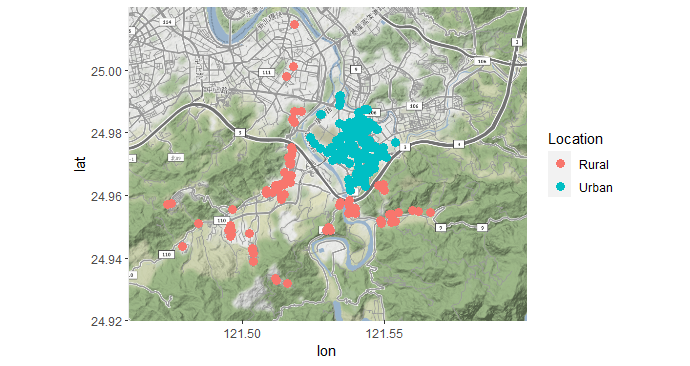
\includegraphics[scale=0.80]{img/regions.png}
    \caption{Xindian District divided into regions}
    \label{fig:regions}
\end{figure}

\begin{figure}[hbt!]
    \centering
    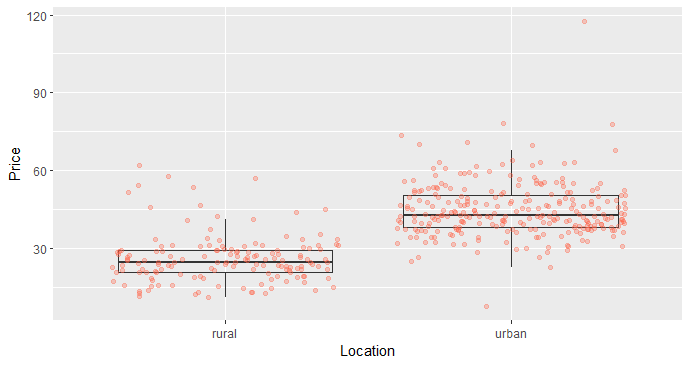
\includegraphics[scale=0.75]{img/boxplot.png}
    \caption{(non log) ppua distributions by location}
    \label{fig:boxplot}
\end{figure}

\begin{figure}[hbt!]
    \centering
    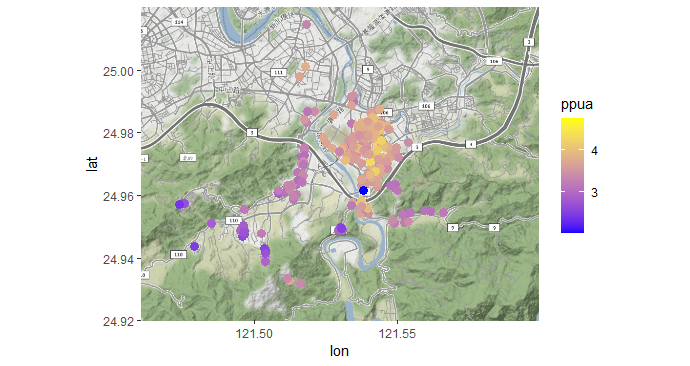
\includegraphics[scale=0.80]{img/ppuamap.png}
    \caption{Xindian district by ppua}
    \label{fig:ppuamap}
\end{figure}

% Seasonal
\begin{figure}[hbt!]
    \centering
    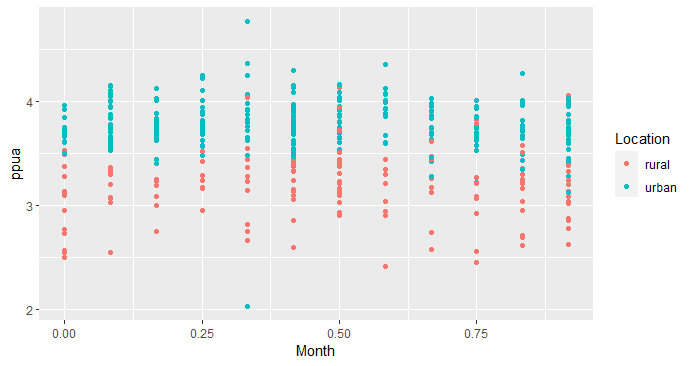
\includegraphics[scale=0.80]{img/seasonal.png}
    \caption{ppua by month}
    \label{fig:seasonal}
\end{figure}

\begin{figure}[hbt!]
    \centering
    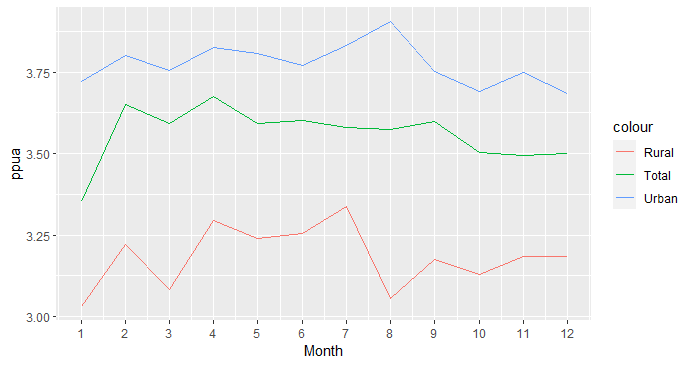
\includegraphics[scale=0.80]{img/seasonalmean.png}
    \caption{mean ppua by month}
    \label{fig:seasonalmean}
\end{figure}

% Age
\begin{figure}[hbt!]
    \centering
    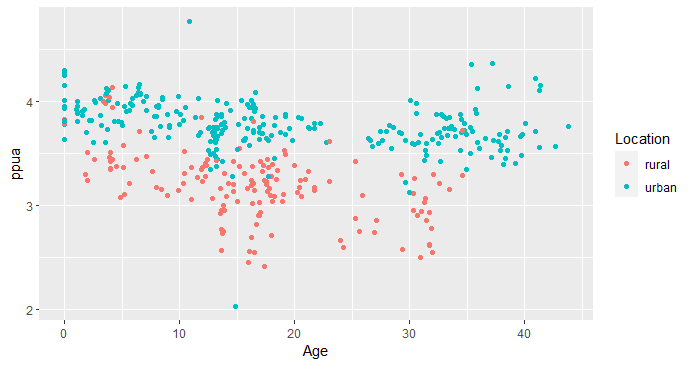
\includegraphics[scale=0.80]{img/agetogether.png}
    \caption{ppua vs age}
    \label{fig:age}
\end{figure}

% \begin{figure}[ht]
%     \centering
%     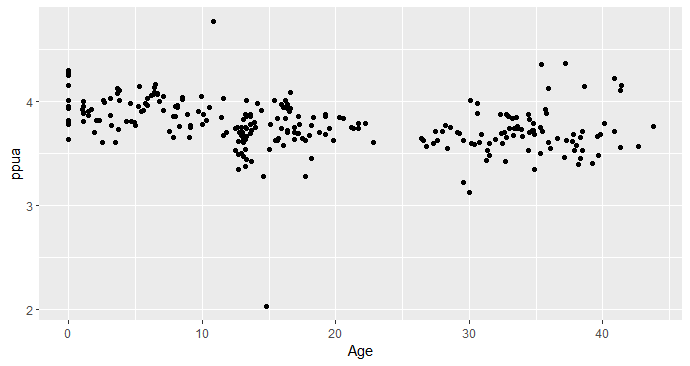
\includegraphics[scale=0.80]{img/ageurban.png}
%     \caption{ppua vs age for urban homes}
%     \label{fig:ageurban}
% \end{figure}

% \begin{figure}[ht]
%     \centering
%     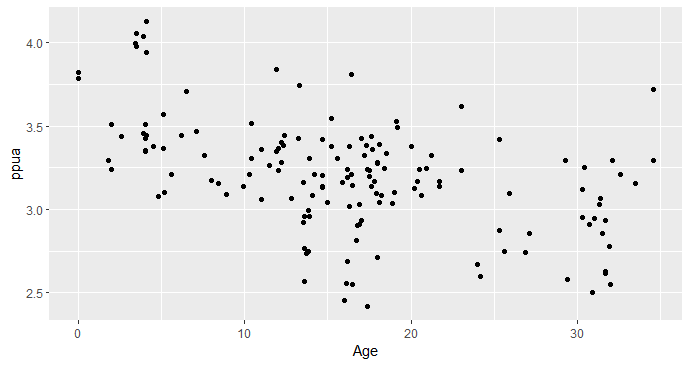
\includegraphics[scale=0.80]{img/agerural.png}
%     \caption{ppua vs age for rural homes}
%     \label{fig:agerural}
% \end{figure}

% MRT
\begin{figure}[hbt!]
    \centering
    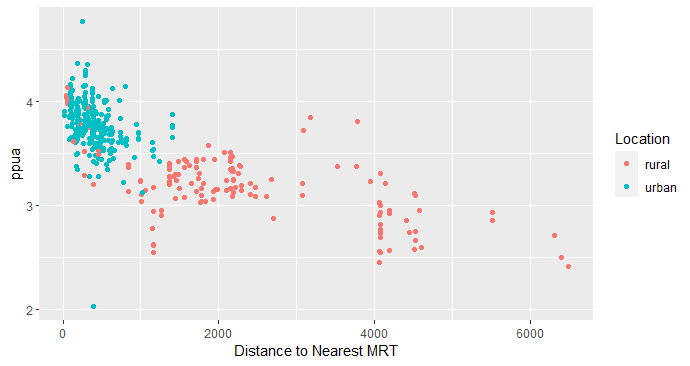
\includegraphics[scale=0.80]{img/mrttogether.png}
    \caption{ppua vs distance to the near mrt}
    \label{fig:mrt}
\end{figure}

% \begin{figure}[ht]
%     \centering
%     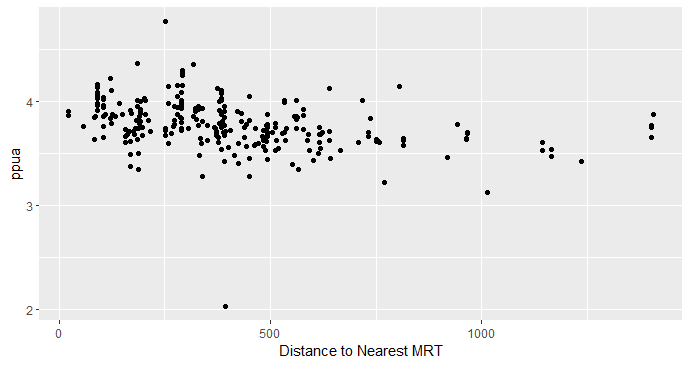
\includegraphics[scale=0.80]{img/mrturban.png}
%     \caption{ppua vs distance to the near mrt for urban homes}
%     \label{fig:mrturban}
% \end{figure}

% \begin{figure}[ht]
%     \centering
%     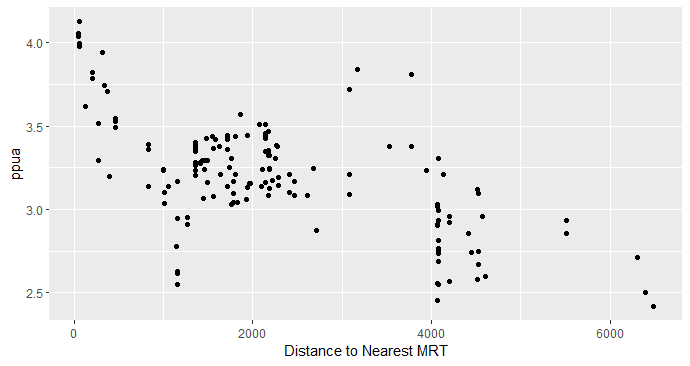
\includegraphics[scale=0.80]{img/mrtrural.png}
%     \caption{ppua vs distance to the near mrt for rural homes}
%     \label{fig:mrtrural}
% \end{figure}

% Stores 
\begin{figure}[hbt!]
    \centering
    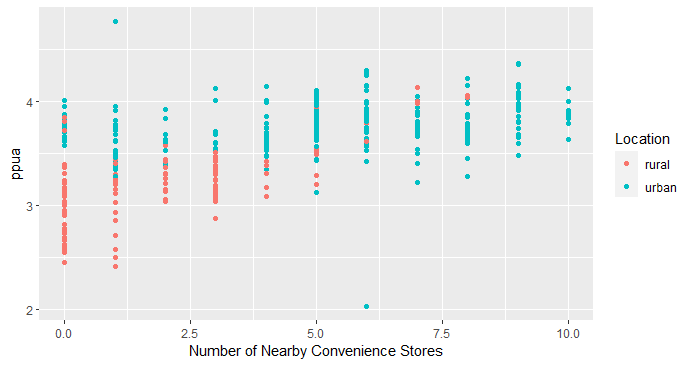
\includegraphics[scale=0.80]{img/storestogether.png}
    \caption{ppua vs number of nearby convenience stores}
    \label{fig:stores}
\end{figure}

% \begin{figure}[ht]
%     \centering
%     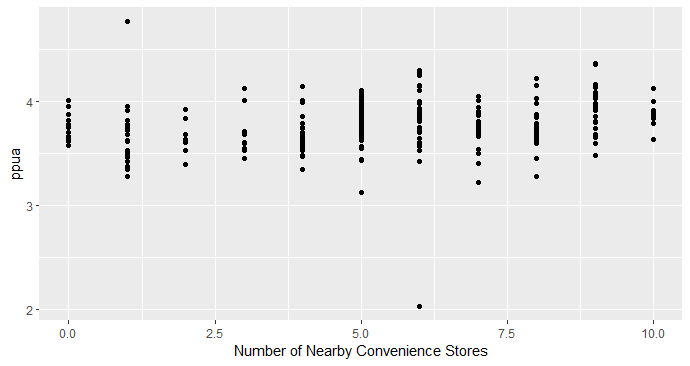
\includegraphics[scale=0.80]{img/storesurban.png}
%     \caption{ppua vs number of nearby convenience stores for urban homes}
%     \label{fig:storesurban}
% \end{figure}

% \begin{figure}[ht]
%     \centering
%     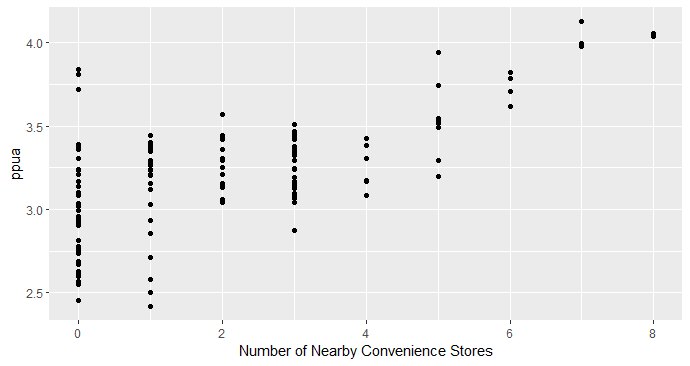
\includegraphics[scale=0.80]{img/storesrural.png}
%     \caption{ppua vs number of nearby convenience stores for rural homes}
%     \label{fig:storesrural}
% \end{figure}

\begin{figure}[hbt!]
    \centering
    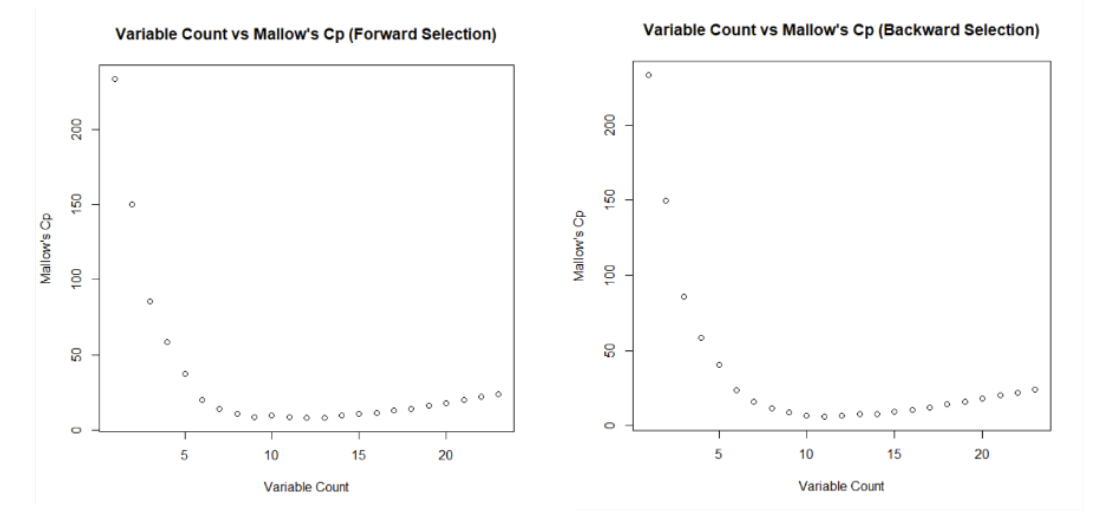
\includegraphics[scale=0.34]{img/mallowcp.png}
    \caption{Mallow's Cp for forward and backward selection}
    \label{fig:mallowcp}
\end{figure}

\begin{figure}[hbt!]
    \centering
    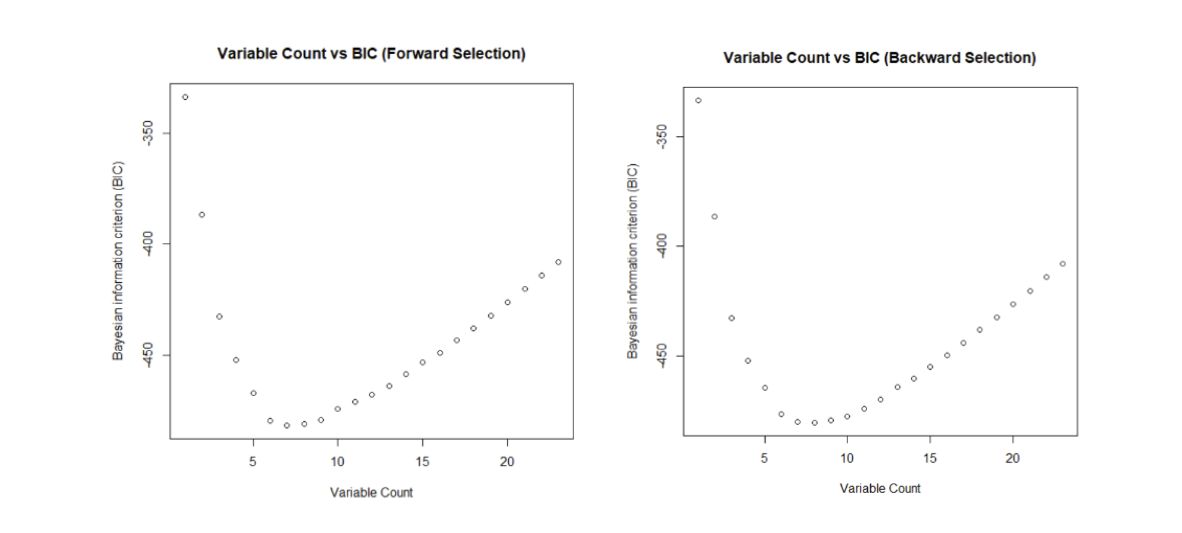
\includegraphics[scale=0.35]{img/bic.png}
    \caption{BIC for forward and backward selection}
    \label{fig:bic}
\end{figure}

\begin{figure}[hbt!]
    \centering
    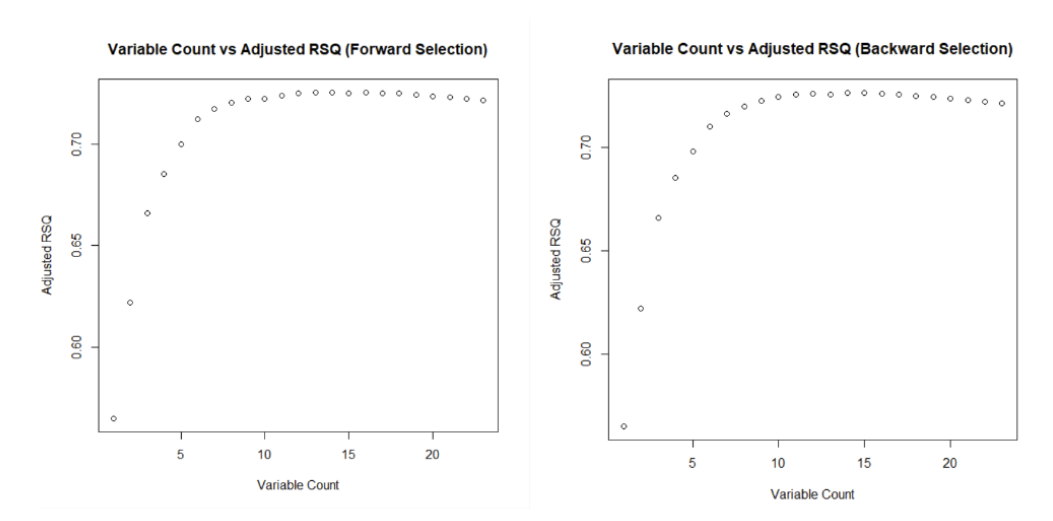
\includegraphics[scale=0.37]{img/rsq.png}
    \caption{Adjusted $R^2$ for forward and backward selection}
    \label{fig:rsq}
\end{figure}

\begin{figure}[hbt!]
    \centering
    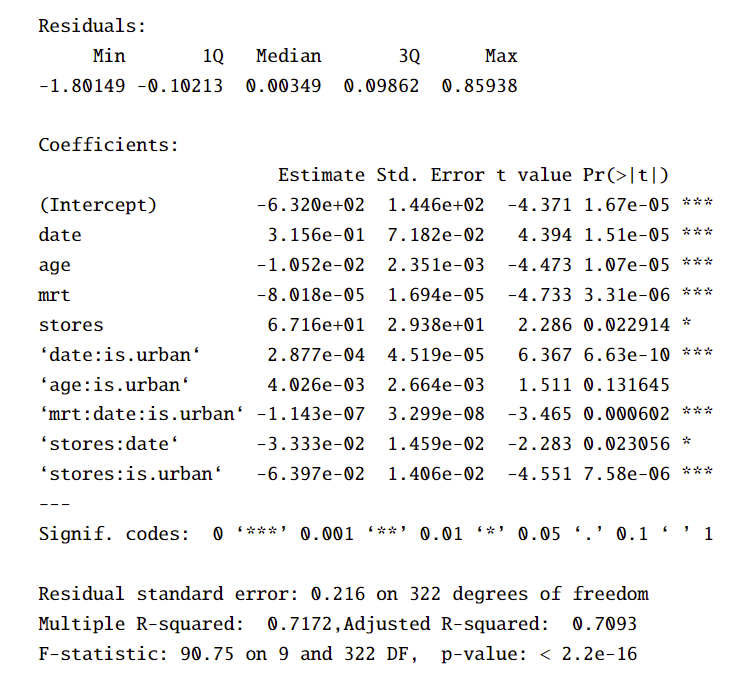
\includegraphics[scale=0.7]{img/summary.png}
    \caption{Summary of the best model}
    \label{fig:summary}
\end{figure}

\begin{figure}[hbt!]
    \centering
    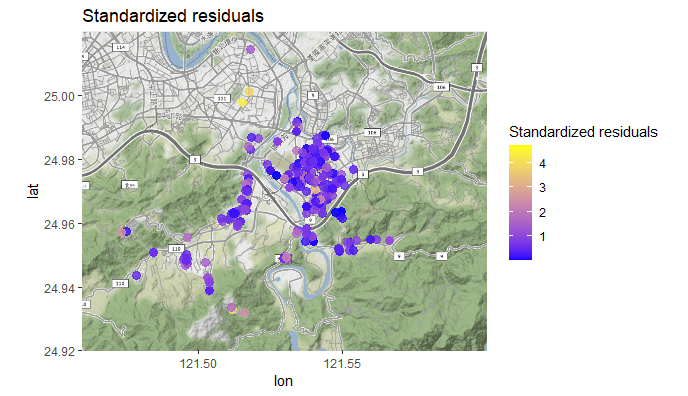
\includegraphics[scale=0.80]{img/standres.png}
    \caption{Standardized residuals}
    \label{fig:standres}
\end{figure}

\begin{figure}[hbt!]
    \centering
    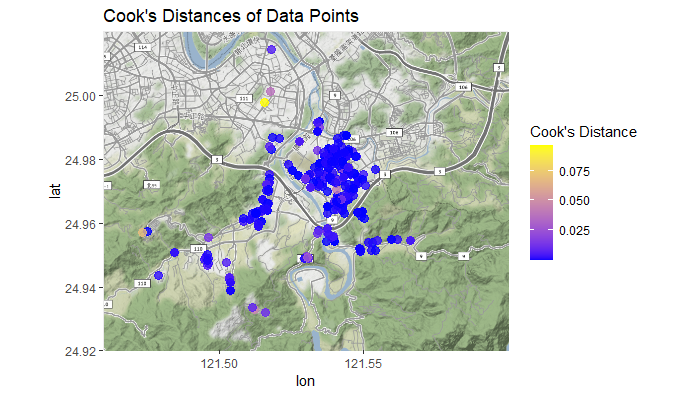
\includegraphics[scale=0.80]{img/cook.png}
    \caption{Cook's distance}
    \label{fig:cook}
\end{figure}

\begin{figure}[hbt!]
    \centering
    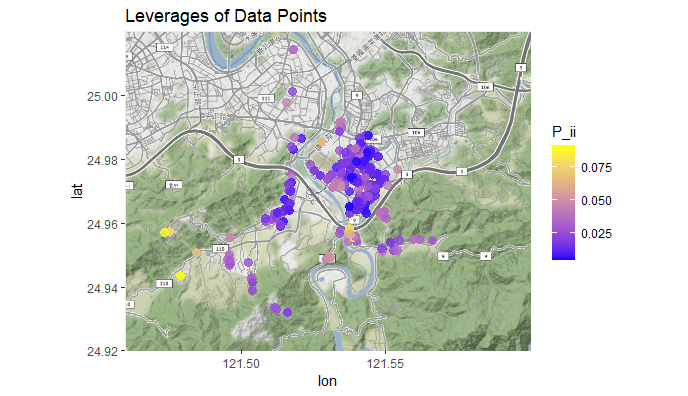
\includegraphics[scale=0.80]{img/lev.png}
    \caption{Leverage}
    \label{fig:lev}
\end{figure}

\begin{figure}[hbt!]
    \centering
    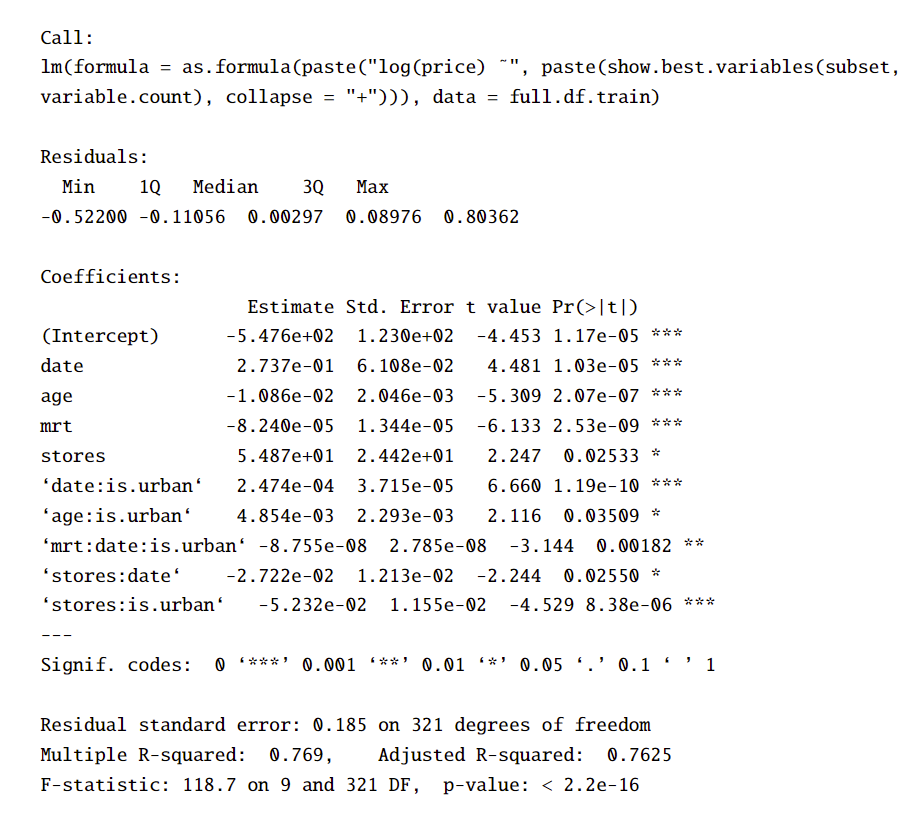
\includegraphics[scale=0.65]{img/n=413.png}
    \caption{Summary of the best model after removing the most extreme outliers}
    \label{fig:n=413}
\end{figure}

\begin{figure}[hbt!]
    \centering
    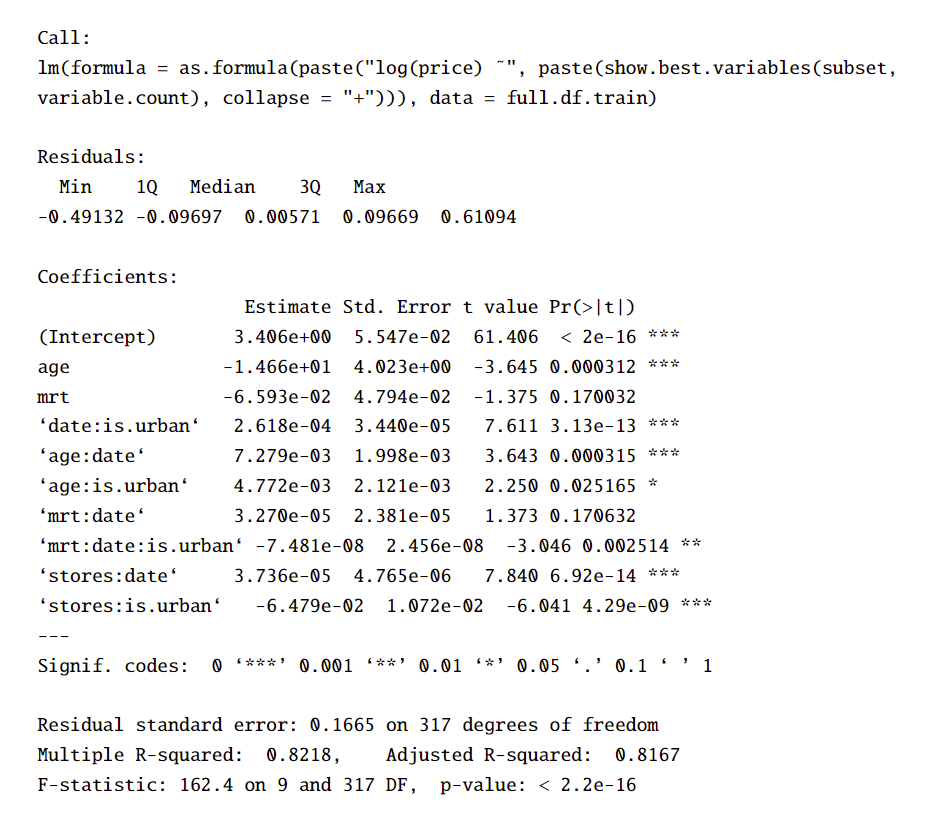
\includegraphics[scale=0.65]{img/n=408.png}
    \caption{Summary of the best model after removing all outliers}
    \label{fig:n=408}
\end{figure}

\clearpage 